\documentclass[12pt, oneside]{article}

\usepackage[letterpaper, scale=0.89, centering]{geometry}
\usepackage{fancyhdr}
\setlength{\parindent}{0em}
\setlength{\parskip}{1em}

\usepackage{tikz}
\usetikzlibrary{automata,positioning,arrows}

\pagestyle{fancy}
\fancyhf{}
\renewcommand{\headrulewidth}{0pt}
\rfoot{\href{https://creativecommons.org/licenses/by-nc-sa/2.0/}{CC BY-NC-SA 2.0} Version \today~(\thepage)}

\usepackage{amssymb,amsmath,pifont,amsfonts,comment,enumerate,enumitem}
\usepackage{currfile,xstring,hyperref,tabularx,graphicx,wasysym}
\usepackage[labelformat=empty]{caption}
\usepackage{xcolor}
\usepackage{multicol,multirow,array,listings,tabularx,lastpage,textcomp,booktabs}

\lstnewenvironment{algorithm}[1][] {   
    \lstset{ mathescape=true,
        frame=tB,
        numbers=left, 
        numberstyle=\tiny,
        basicstyle=\rmfamily\scriptsize, 
        keywordstyle=\color{black}\bfseries,
        keywords={,procedure, div, for, to, input, output, return, datatype, function, in, if, else, foreach, while, begin, end, }
        numbers=left,
        xleftmargin=.04\textwidth,
        #1
    }
}
{}

\newcommand\abs[1]{\lvert~#1~\rvert}
\newcommand{\st}{\mid}

\newcommand{\cmark}{\ding{51}}
\newcommand{\xmark}{\ding{55}}
 
\begin{document}
\begin{flushright}
    \StrBefore{\currfilename}{.}
\end{flushright} 
\subsection*{Week 5 at a glance}

\subsubsection*{Textbook reading: Chapter 2}

\vspace{-20pt}

Before Monday, read Introduction to Section 2.1 (pages 101-102).

Before Wednesday, read Section 2.1

Before Friday, read Theorem 2.20.

For Week 6 Monday: Page 165-166 Introduction to Section 3.1.

\vspace{-20pt}

\subsubsection*{We will be learning and practicing to:}
\vspace{-20pt}

\begin{itemize}
    \item Clearly and unambiguously communicate computational ideas using appropriate formalism. Translate across levels of abstraction.
    \begin{itemize}
        \item Describe and use models of computation that don't involve state machines.
        \begin{itemize}
            \item {\bf Identify the components of a formal definition of a context-free grammar (CFG)}
            \item {\bf Derive strings in the language of a given CFG}
            \item {\bf Determine the language of a given CFG}
            \item {\bf Design a CFG generating a given language}
            \item {\bf Use context-free grammars and relate them to languages and pushdown automata.}
        \end{itemize}
        \item Use precise notation to formally define the state diagram of a Turing machine
        \item Use clear English to describe computations of Turing machines informally.
        \begin{itemize}
            \item {\bf Design a PDA that recognizes a given language.}
         \end{itemize}
       \item Give examples of sets that are context-free (and prove that they are).
       \begin{itemize}
          \item {\bf State the definition of the class of context-free languages}
          \item {\bf Explain the limits of the class of context-free languages}
          \item {\bf Identify some context-free sets and some non-context-free sets}
       \end{itemize}
    \end{itemize}
    \item Know, select and apply appropriate computing knowledge and problem-solving techniques. 
    Reason about computation and systems.
    \begin{itemize}
        \item Describe and prove closure properties of classes of languages under certain operations.
        \begin{itemize}
            \item {\bf Apply a general construction to create a new PDA or CFG from an example one.}
            \item {\bf Formalize a general construction from an informal description of it.}
            \item {\bf Use general constructions to prove closure properties of the class of context-free langugages.}
            \item {\bf Use counterexamples to prove non-closure properties of the class of context-free langugages.}
        \end{itemize}
    \end{itemize}
\end{itemize}

\vspace{-20pt}

\subsubsection*{TODO:}
\begin{list}{\itemsep-10pt}
   \item Schedule your Test 1 Attempt 1, Test 2 Attempt 1, Test 1 Attempt 2, and Test 2 Attempt 2 times
   at PrairieTest (http://us.prairietest.com) . The first Test 1 sessions are next week!
   \item Review Quiz 4 on PrairieLearn (http://us.prairielearn.com), due 2/5/2025
   \item Homework 3 submitted via Gradescope (https://www.gradescope.com/), due 2/6/2025
   \item Review Quiz 5 on PrairieLearn (http://us.prairielearn.com), due 2/12/2025
\end{list}

\newpage



\newpage
\subsection*{Monday: More Pushdown Automata}




{\bf Definition} A {\bf pushdown automaton} (PDA) is  specified by a  $6$-tuple $(Q, \Sigma, \Gamma, \delta, q_0, F)$
where $Q$ is the finite set of states, $\Sigma$ is the input alphabet,  $\Gamma$ is the stack alphabet,
\[
    \delta: Q \times \Sigma_\varepsilon  \times  \Gamma_\varepsilon \to \mathcal{P}( Q \times \Gamma_\varepsilon)
\]
is the transition function,  $q_0 \in Q$ is the start state, $F \subseteq  Q$ is the set of accept states.










For the PDA state diagrams below, $\Sigma = \{0,1\}$.

\vspace{-15pt}

\begin{center}
\begin{tabular}{c c}
Mathematical description of language & State diagram of PDA recognizing language\\
\hline
& $\Gamma = \{ \$, \#\}$ \hspace{2.3in} \\
& \\
& 
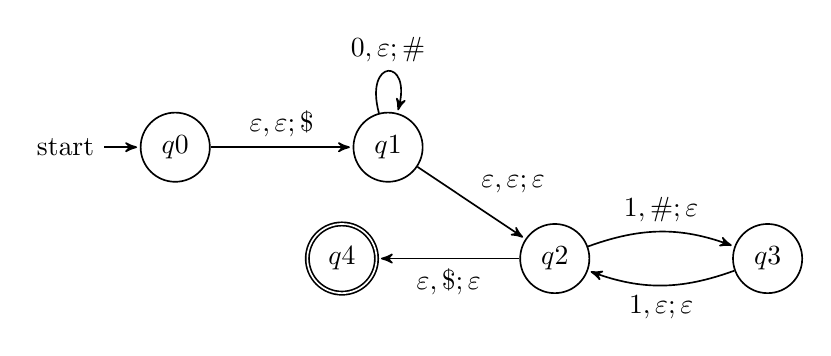
\begin{tikzpicture}[->,>=stealth',shorten >=1pt, auto, node distance=2cm, semithick]
    \tikzstyle{every state}=[text=black, fill=none]
    
    \node[initial,state] (q0)          {$q0$};
    \node[state]         (q1) [right of=q0, xshift=20pt] {$q1$};
    \node[state]         (q2) [below right of=q1, xshift=20pt] {$q2$};
    \node[state]         (q3) [right of=q2, xshift=20pt] {$q3$};
    \node[state,accepting]         (q4) [left of=q2, xshift=-20pt] {$q4$};
    
    \path (q0) edge [bend left=0] node {$\varepsilon, \varepsilon; \$$} (q1)
        (q1) edge  [loop above] node {$0, \varepsilon; \#$} (q1)
        (q1) edge [bend left=0] node {$\varepsilon, \varepsilon; \varepsilon$} (q2)
        (q2) edge  [bend left=20] node [midway, above] {$1, \#; \varepsilon$} (q3)
        (q3) edge  [bend left=20] node [midway, below] {$1, \varepsilon; \varepsilon$} (q2)
        (q2) edge  [bend left=0] node {$\varepsilon, \$; \varepsilon$} (q4)
    ;
\end{tikzpicture}
\\
& \\
& \\
\hline
& $\Gamma = \{ \sun, 1\}$ \hspace{2.3in} \\
& \\
& 
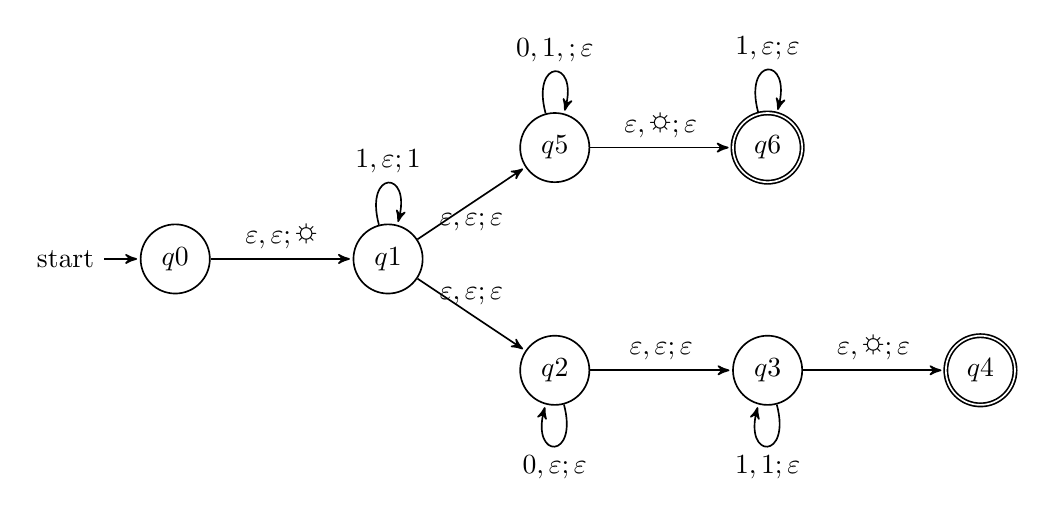
\begin{tikzpicture}[->,>=stealth',shorten >=1pt, auto, node distance=2cm, semithick]
    \tikzstyle{every state}=[text=black, fill=none]
    
    \node[initial,state] (q0)          {$q0$};
    \node[state]         (q1) [right of=q0, xshift=20pt] {$q1$};
    \node[state]         (q2) [below right of=q1, xshift=20pt] {$q2$};
    \node[state]         (q3) [right of=q2, xshift=20pt] {$q3$};
    \node[state,accepting]  (q4) [right of=q3, xshift=20pt] {$q4$};
    \node[state]         (q5) [above right of=q1, xshift=20pt] {$q5$};
    \node[state,accepting]  (q6) [right of=q5, xshift=20pt] {$q6$};
    
    \path (q0) edge [bend left=0] node {$\varepsilon, \varepsilon; \sun$} (q1)
        (q1) edge  [loop above] node {$1, \varepsilon; 1$} (q1)
        (q1) edge [bend left=0] node [below] {$\varepsilon, \varepsilon; \varepsilon$} (q5)
        (q1) edge [bend left=0] node [above]{$\varepsilon, \varepsilon; \varepsilon$} (q2)
        (q5) edge [loop above] node {$0, 1, ; \varepsilon$} (q5)
        (q5) edge [bend left=0] node {$\varepsilon, \sun; \varepsilon$} (q6)
        (q6) edge [loop above] node {$1, \varepsilon; \varepsilon$} (q6)
        (q2) edge [loop below] node {$0, \varepsilon; \varepsilon$} (q2)
        (q2) edge  [bend left=0] node {$\varepsilon, \varepsilon; \varepsilon$} (q3)
        (q3) edge  [loop below] node {$1, 1; \varepsilon$} (q3)
        (q3) edge  [bend left=0] node {$\varepsilon, \sun; \varepsilon$} (q4)
    ;
\end{tikzpicture}
\\
& \\
& \\
\hline
& \\
& \\
& \\
$\{ 0^i 1^j 0^k \mid i,j,k \geq 0 \}$ & \\
& \\
& \\

\end{tabular}
\end{center}
{\it Note: alternate notation is to replace $;$ with $\to$ on arrow labels.}

\newpage
Corollary: for each language $L$ over $\Sigma$, if there is an NFA $N$ with $L(N)=L$
then there is a PDA $M$ with $L(M) = L$

Proof idea: Declare stack alphabet to be $\Gamma = \Sigma$ and then 
don't use stack at all. 


 \vfill

\begin{comment}
{\it Extra practice}: Consider the state diagram of a PDA with input alphabet 
$\Sigma$ and stack alphabet $\Gamma$.

\begin{center}
\begin{tabular}{|c|c|}
\hline
Label & means \\
\hline
$a, b ; c$ when $a \in \Sigma$, $b\in \Gamma$, $c \in \Gamma$ 
& \hspace{3in} \\
& \\
& \\
& \\
& \\
&\\
\hline
$a, \varepsilon ; c$ when $a \in \Sigma$, $c \in \Gamma$ 
& \hspace{3in} \\
& \\
& \\
& \\
& \\
&\\
\hline
$a, b ; \varepsilon$ when $a \in \Sigma$, $b\in \Gamma$
& \hspace{3in} \\
& \\
& \\
& \\
& \\
&\\
\hline
$a, \varepsilon ; \varepsilon$ when $a \in \Sigma$
& \hspace{3in} \\
& \\
& \\
& \\
& \\
&\\
\hline
\end{tabular}
\end{center}


How does the meaning change if $a$ is replaced by $\varepsilon$?
\end{comment}

{\it Big picture}: PDAs are motivated by wanting to add some memory of unbounded size to NFA. How 
do we accomplish a similar enhancement of regular expressions to get a syntactic model that is 
more expressive?

DFA, NFA, PDA: Machines process one input string at a time; the computation of a machine on its input string 
reads the input from left to right.

Regular expressions: Syntactic descriptions of all strings that match a particular pattern; the language 
described by a regular expression is built up recursively according to the expression's syntax

{\bf Context-free grammars}: Rules to produce one string at a time, adding characters from the middle, beginning, 
or end of the final string as the derivation proceeds.\\

\vfill
 
\newpage
\section*{Wednesday: Context-free Grammars and Languages}





Definitions below are on pages 101-102.

\vspace{-20pt}

\begin{center}
    \begin{tabular}{|p{2.4in}cp{3.6in}|}
    \hline 
    {\bf Term} & {\bf Typical symbol} & {\bf Meaning} \\
     & or {\bf Notation} & \\
    \hline
    \hline
    {\bf Context-free grammar} (CFG) & $G$ & $G = (V, \Sigma, R, S)$ \\
    The set of {\bf variables}& $V$ & Finite  set of symbols that represent phases in production pattern\\
    The set of {\bf terminals} & $\Sigma$ & Alphabet of symbols of strings generated  by CFG \\
    & & $V \cap \Sigma = \emptyset$ \\
    The set of {\bf rules}& $R$ & Each rule is  $A \to u$ with $A \in V$ and $u  \in (V  \cup \Sigma)^*$\\
    The {\bf start} variable&  $S$  & Usually  on left-hand-side of first/ topmost rule \\
    & &\\
    {\bf Derivation} & $S \Rightarrow \cdots \Rightarrow w$& 
    Sequence  of substitutions in a  CFG (also written $S \Rightarrow^* w$). At each step, we can apply one rule 
    to one occurrence of a variable in the current string by substituting that occurrence of the variable with the 
    right-hand-side of the rule. The derivation must end when the current string has only terminals (no variables)
    because then there are no instances of variables to apply a rule to.\\
    Language {\bf generated} by the context-free grammar $G$ & $L(G)$ &The set of strings for which there is a derivation in $G$. 
    Symbolically: $\{  w \in \Sigma^* \mid S \Rightarrow^* w \}$ i.e. $$\{  w \in \Sigma^* \mid \text{there is  derivation in $G$ that ends
    in $w$} \}$$\\
    {\bf Context-free language} & & A language that is the language generated by some context-free grammar\\
    \hline
    \end{tabular}
\end{center}

\vfill

  
{\bf Examples of context-free grammars, derivations in those grammars, and the languages generated by those grammars}
  
$G_1 =  (\{S\}, \{0\}, R, S)$ with rules
  \begin{align*}
    &S \to 0S\\
    &S \to 0\\
  \end{align*}
  In  $L(G_1)$ \ldots 
  
\vfill

  Not in $L(G_1)$ \ldots 


\vfill

\newpage
  $G_2 =  (\{S\}, \{0,1\}, R, S)$
  \[
  S \to 0S \mid 1S \mid \varepsilon
  \]
  In  $L(G_2)$ \ldots 
  
  \vfill
  
  Not in $L(G_2)$ \ldots 

  \vfill

  $(\{S, T\}, \{0, 1\}, R, S)$ with  rules
  \begin{align*}
  &S \to T1T1T1T \\
  &T \to  0T \mid 1T \mid \varepsilon
  \end{align*}

  In  $L(G_3)$ \ldots 
  
  \vfill
  
  Not in $L(G_3)$ \ldots 

  \vfill

  $G_4 =  (\{A, B\}, \{0, 1\}, R, A)$ with rules
  \[
    A \to 0A0 \mid  0A1 \mid 1A0  \mid 1A1 \mid  1
  \]
  In  $L(G_4)$ \ldots 
  
  \vfill
  
  Not in $L(G_4)$ \ldots 

  \vfill

  
  \newpage
  Design a CFG to generate the  language $\{a^n b^n \mid  n  \geq  0\}$
  
  
  \vfill 


  Design a CFG to generate the  language $\{a^i b^j \mid j \geq i  \geq 0\}$
  
  \vfill
  
  Design a PDA to recognize the  language $\{a^i b^j \mid j \geq i  \geq 0\}$
  
  
  \vfill
  \newpage     
\newpage
\subsection*{Friday: Context-free and non-context-free languages}




{\bf Theorem  2.20}: A language is  generated by some context-free  grammar
if  and only if it is recognized by some push-down automaton.

Definition: a language is called {\bf context-free} if it is the language generated by a context-free grammar.
The class of all context-free language over a given alphabet $\Sigma$ is called {\bf CFL}.

Consequences:
\begin{itemize}
    \item Quick proof that every regular language is context free 
    \item To prove closure of the class of context-free languages under a given operation, we can choose 
    either of two modes 
    of proof (via CFGs or PDAs) depending on which is easier
    \item To fully specify a PDA we could give its $6$-tuple formal definition or we could give its input 
alphabet, stack alphabet, and state diagram.
An informal description of a PDA is a step-by-step description of how its computations 
would process input strings; the reader should be able to reconstruct the state diagram or formal 
definition precisely from such a descripton. The informal description of a PDA can refer to some 
common modules or subroutines that are computable by PDAs:
\begin{itemize}
  \item PDAs can ``test for emptiness of stack'' without providing details. 
  {\it How?} We can always push a special end-of-stack symbol, $\$$, at the start, before processing
  any input, and then use this symbol as a flag.
  \item PDAs can ``test for end of input'' without providing details.
  {\it How?} We can transform a PDA to one where accepting states are only those reachable 
  when there are no more input symbols.
\end{itemize}

\end{itemize}




\vfill

\newpage
Suppose $L_1$ and $L_2$ are context-free languages over $\Sigma$.  {\bf Goal}:  $L_1 \cup L_2$  is  also context-free.

{\it Approach 1: with  PDAs}

Let $M_1 = ( Q_1, \Sigma, \Gamma_1, \delta_1, q_1, F_1)$ and
$M_2 = ( Q_2, \Sigma, \Gamma_2, \delta_2, q_2, F_2)$ be PDAs with 
$L(M_1) =  L_1$  and  $L(M_2) = L_2$.

Define $M = $

\vfill

{\it Approach  2: with CFGs}

Let $G_1 = (V_1, \Sigma, R_1, S_1)$  and   $G_2 = (V_2, \Sigma, R_2, S_2)$  be CFGs  with
$L(G_1) =  L_1$  and  $L(G_2) = L_2$.

Define $G = $

\vfill

\newpage
Suppose $L_1$ and $L_2$ are context-free languages over $\Sigma$.  {\bf Goal}:  $L_1 \circ L_2$  is  also context-free.


{\it Approach 1: with  PDAs}

Let $M_1 = ( Q_1, \Sigma, \Gamma_1, \delta_1, q_1, F_1)$ and
$M_2 = ( Q_2, \Sigma, \Gamma_2, \delta_2, q_2, F_2)$ be PDAs with 
$L(M_1) =  L_1$  and  $L(M_2) = L_2$.

Define $M = $

\vfill

{\it Approach  2: with CFGs}

Let $G_1 = (V_1, \Sigma, R_1, S_1)$  and   $G_2 = (V_2, \Sigma, R_2, S_2)$  be CFGs  with
$L(G_1) =  L_1$  and  $L(G_2) = L_2$.

Define $G = $

\vfill

{\it Summary}

Over a fixed alphabet $\Sigma$, a language $L$ is {\bf regular}

\vspace{-20pt}
\begin{center}
    iff it is described by some regular expression \\
    iff it is recognized by some DFA\\
    iff it is recognized by some NFA
\end{center}

Over a fixed alphabet $\Sigma$, a language $L$ is {\bf context-free}

\vspace{-20pt}
\begin{center}
    iff it is generated by some CFG\\
    iff it is recognized by some PDA
\end{center}

\vfill

{\bf Fact}: Every regular language is a context-free language.

\vfill

{\bf Fact}: There are context-free languages that are not nonregular.

\vfill

{\bf Fact}: There are countably many regular languages.

\vfill

{\bf Fact}: There are countably infinitely many context-free languages.

\vfill

{\it Consequence}: Most languages are {\bf not} context-free!

\vfill

\newpage
{\bf Examples  of non-context-free languages}

\begin{align*}
    &\{ a^n b^n c^n \mid 0 \leq n , n \in \mathbb{Z}\}\\
    &\{ a^i b^j c^k \mid 0 \leq i \leq j \leq k , i \in \mathbb{Z}, j \in \mathbb{Z}, k \in \mathbb{Z}\}\\
    &\{ ww \mid w \in \{0,1\}^* \}
\end{align*}
(Sipser Ex 2.36, Ex 2.37, 2.38)

There is a Pumping Lemma for CFL that can be used to prove a specific language is non-context-free: 
If $A$ is a context-free language, there
is a number $p$ where, if $s$ is any string in $A$ of length at least $p$, then $s$ may be divided 
into five pieces $s = uvxyz$ where (1) for each $i \geq 0$, $uv^ixy^iz \in A$, (2) $|uv|>0$, (3) $|vxy| \leq p$.
{\it We will not go into the details of the proof or application of Pumping Lemma for CFLs this quarter.}


Recall: A set $X$ is said to be {\bf closed} under an operation $OP$ if, for any elements in $X$, applying 
$OP$ to them gives an element in $X$.  


\begin{center}
\begin{tabular}{|c|l|}
\hline
True/False & Closure claim \\
\hline
True &  The set of integers is closed under multiplication. \\
& $\forall x \forall y \left( ~(x \in \mathbb{Z} \wedge y \in \mathbb{Z})\to xy \in \mathbb{Z}~\right)$ \\
\hline
True & For each set $A$, the power set of $A$ is closed under intersection. \\
& $\forall A_1 \forall A_2 \left( ~(A_1 \in \mathcal{P}(A) \wedge A_2 \in \mathcal{P}(A) \in \mathbb{Z}) \to A_1 \cap A_2 \in \mathcal{P}(A)~\right)$ \\
\hline
  & The class of regular languages over $\Sigma$ is closed under complementation. \\
  & \\
 \hline
  & The class of regular languages over $\Sigma$ is closed under union. \\
  & \\
 \hline
  & The class of regular languages over $\Sigma$ is closed under intersection. \\
  & \\
  \hline
  & The class of regular languages over $\Sigma$ is closed under concatenation. \\
  & \\
 \hline
  & The class of regular languages over $\Sigma$ is closed under Kleene star. \\
  & \\
\hline
    & The class of context-free languages over $\Sigma$ is closed under complementation. \\
  & \\
\hline
    & The class of context-free languages over $\Sigma$ is closed under union. \\
  & \\
\hline
    & The class of context-free languages over $\Sigma$ is closed under intersection. \\
  & \\
\hline
    & The class of context-free languages over $\Sigma$ is closed under concatenation. \\
  & \\
\hline
    & The class of context-free languages over $\Sigma$ is closed under Kleene star. \\
  & \\
\hline
\end{tabular}
\end{center}
 


\end{document}
